
\section{Introduction}


\begin{figure*}
\centering
\subfloat[\Process~$R$ efficiently advertises its content using epidemic propagation. Every \process requests $R$ if needed.\label{fig:partition_intuitionA}]{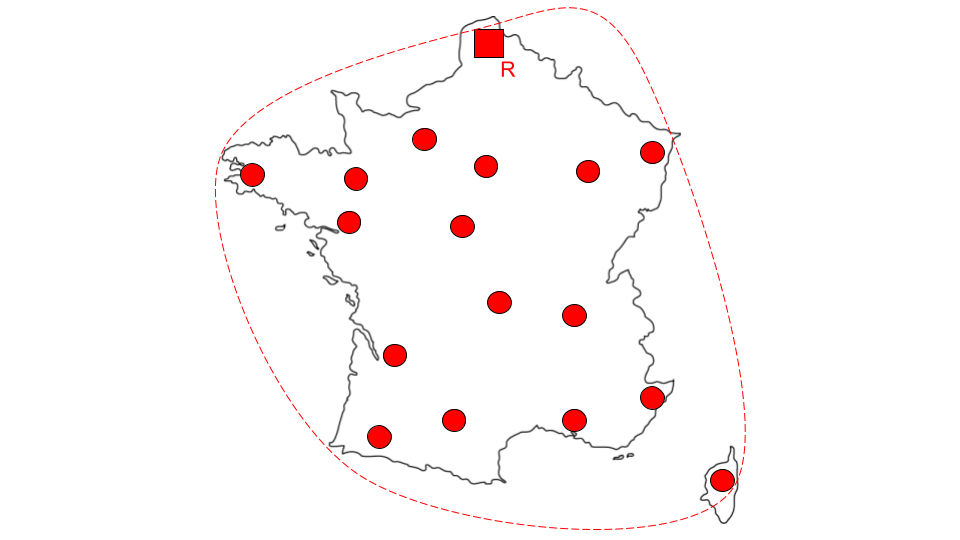
\includegraphics[trim=6cm 0.33cm 6cm 0.33cm, clip, width=0.24\textwidth]{img/Dynamic-partitioning-1.png}}
\hfill
\subfloat[\Process $G$ creates a second replica splitting the red set in two. \Processes request their closest replica host.\label{fig:partition_intuitionB}]{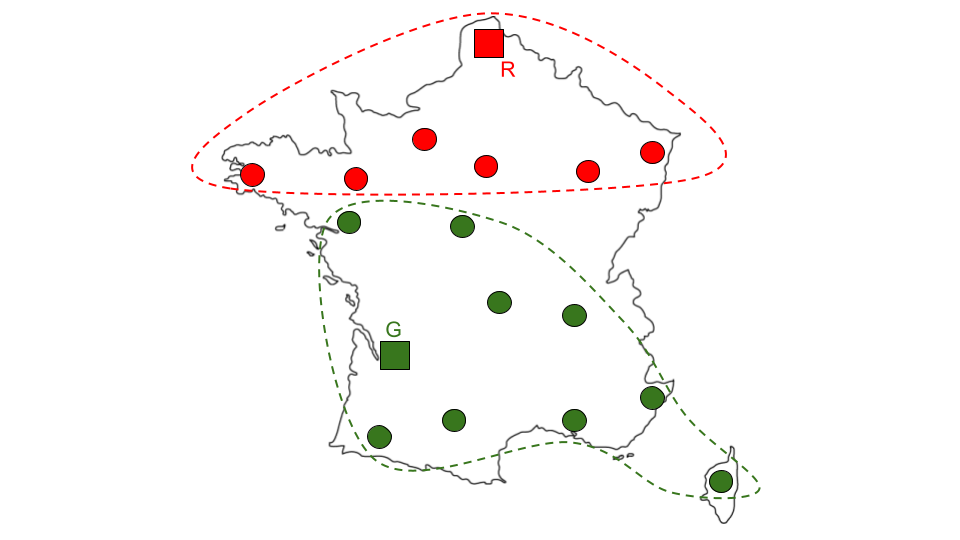
\includegraphics[trim=6cm 0.33cm 6cm 0.33cm, clip, width=0.24\textwidth]{img/Dynamic-partitioning-2.png}}\hfill
\subfloat[\Process $B$ creates another replica. \Process~$B$ needs to notify only a small subset of \processes.\label{fig:partition_intuitionC}]{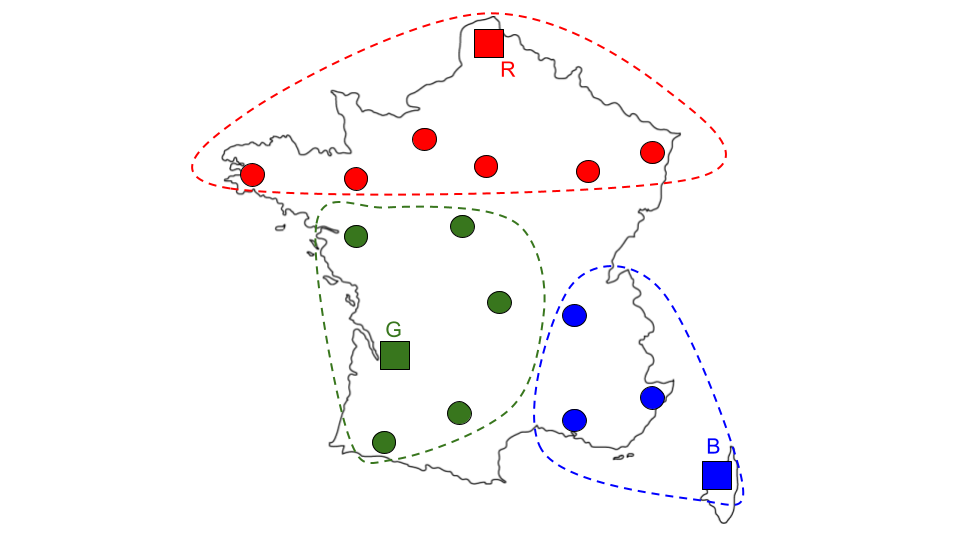
\includegraphics[trim=6cm 0.33cm 6cm 0.33cm, clip, width=0.24\textwidth]{img/Dynamic-partitioning-3.png}}\hfill
\subfloat[\Process $G$ destroys its replica. \Processes that belong to its partition must find the closest partition they are in.\label{fig:partition_intuitionD}]{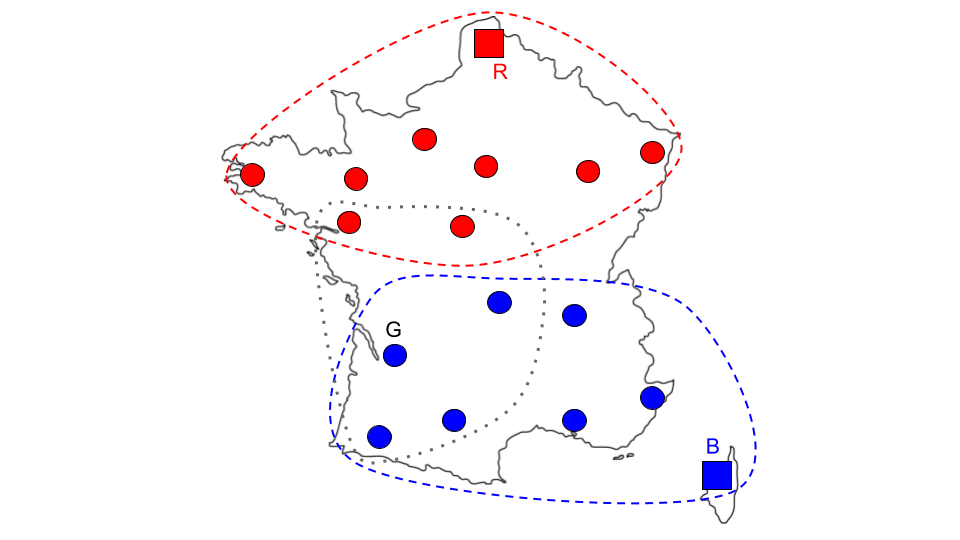
\includegraphics[trim=6cm 0.33cm 6cm 0.33cm, clip, width=0.24\textwidth]{img/Dynamic-partitioning-4.png}}
%
\caption{The french RENATER topology. Partitions
  grow and shrink depending on creations and removals of
  replicas.} \label{fig:partition_intuition}
\end{figure*}

%%% Local Variables: 
%%% mode: latex
%%% TeX-master: "../paper"
%%% ispell-local-dictionary: "english"
%%% End: 
 %% positioning

In recent years, the data storage paradigm shifted from centralized in
the cloud to distributed at the edges of the network. 
% There is an ongoing evolution of storing data from the cloud to the
% edges of the network.
This shift aims at keeping the data close to
\begin{inparaenum}[(i)]
\item its producers since data may be too expensive or sensitive to be
  transmitted through the network; and
\item its consumers so data may quickly and efficiently reach
  them~\cite{cachier, foggy_cache, shi2016edge}.
\end{inparaenum}
%% It avoids transmitting Either because it is where it has been
%% created and it is too expensive to be transmitted through the
%% network, or because it has been replicated to bring data closer to
%% the end users ~\cite{shi2016edge, foggy_cache, cachier}.
%
To favour this transition, new designs for data management across Edge
infrastructures have been investigated~\cite{confais2017object,
  confais2017performance, fogstore, hasenburg2020towards}.  They
enable strategies to confine traffic by writing data locally and
replicating content according to effective needs. However, locating
content remains challenging. Retrieving a content location may
actually take more time than retrieving the content itself.
%% Although
%% these systems, provide good properties such as favouring network
%% traffic confinement by writting data locally and replicating contents
%% according to the effective needs, determining the location where to
%% get the content might be more expensive than retrieving the content
%% itself.
%
Indeed, these systems, when not using a centralized index hosted in a
Cloud~\REF, rely on distributed hash
tables~\cite{maymounkov2002kademlia} spread across the different
\processes composing the infrastructure. When a client wants to access
specific content, it requests a remote \process to provide at least
one \process identity to retrieve this content from. After it
retrieved the content, the client can create another replica to
improve the performance of future accesses, but it must contact the
content indexing service again to notify of such change.
%% a local replica is created to improve the performance for future
%% accesses and the process in charge of maintaining the index is
%% contacted once again to reflect this new location.
%

%This strategy has two majors drawbacks :
%\begin{itemize}
%  \item (i) the lookup penalty: the network latency to reach this
%    remote node incurs an additional delay~\cite{asrese2019measuring,
%      doan2019tracing} to get the object before
%    being able to start its downloading ;
%  \item (ii) the selection of the node(s) from which the content is
%    returned: due to the lack of information that would allow the  a request to each process storing a
%%    replica is perfomed in
%\end{itemize}

These approaches directly contradict with the objectives of Edge
infrastructures that aim at reducing the impact of latency as well as
the volume of data passing through the network.
%
First, accessing a remote \node to request content location(s) raises
hot spots and availability issues. But most importantly, it results in
additional delays that occur even before the actual download
started~\cite{asrese2019measuring, doan2019tracing}.
%
Second, the client gets a list of content locations at the discretion
of content indexing services. Without information about these
locations, it often ends up downloading from multiple replica hosts,
yet only keeping the fastest answer~\REF. In turns, either a client wastes
network resources, or faces lower response time.
%% there is no information to select the ``best'' node among the possible
%% candidates from which the content could be retrieved. In most cases,
%% this results in parallel requests performed by the client node to each
%% candidate with the goal of retrieving the content as efficient as
%% possible.


A ``simple'' way to tackle the aforementioned limitations would be to
maintain on each node composing the infrastructure and for each
content, an index of all replicas (and their ``distance'').  In such
an approach, each time a new replica is created or deleted, a message
is broadcasted from the node that performed the operation (\ie the
source) to all nodes, increasing the distance information at each hop.
%
In addition to being complicated for large-scale systems, maintaining
a global view on each node is useless as there is no interest to
inform a node of the creation/removal of a replica at the opposite of
the network (each node trying to get content from the ``closest''
one).  In other words, the broadcast should be limited to a partition
of the infrastructure, (\ie the subset of nodes that has to update the
current location for this particular content). Obviously, these
partitions depend and evolve according to concurrent operations made
by nodes (replica creation/removal) as well as dynamic changes in the
infrastructure (network failures, node apparitions/leaves).

In this paper, we propose a first implementation of such a protocol.
Entitled Adaptive Scoped broadcast (\NAME), 
our protocol relies on a primitive that forwards
messages until a certain condition is reached, \ie the scope. The
scope is defined by a boolean function (predicate) that returns
whether a message should be propagated or not around its
broadcaster. In the current scenario, the stop condition is related to
the distance to the nearest replica : if the message that a node receives
indicates a content has a longer distance than that which the node
knows then the transfer of the message is useless and so stopped.
%
This primitive is used to guarantee that eventually, every node knows
its best partition, hence its closest replica, despite concurrent
events and receipt orders. Overall, \NAME is a wait-free reactive protocol for
dynamic logical partitioning.  Its overhead actually depends on
its operations and current partitions in the system. When the system
becomes quiescent, nodes eventually converge to their respective
partition and do not require further communication afterward.

\TODO{talk about the proof}

We evaluated our protocol through two simulation scenarios using
\textit{Peersim}~\cite{montresor2009peersim}. First, we confirm that
\NAME allow consistent partitioning in an ad-hoc network composed of
10K nodes.  Second, we illustrate how \NAME enables the lock down of
the traffic in dynamic inter autonomous systems.  More precisely, we
simulated a worldwilde infrastructure by duplicating the GEANT
topology - a real infrastructure spanning across Europe – and by
connecting these two clusters with a high latency link: 200 ms
simulating cross-continental communications such as Europe-America.

%
\begin{figure*}
  \newcommand{\SCALE}{0.95} %% scale of sub figures
  \newcommand\X{50pt}
  \newcommand\Y{-50pt}
  
  \newcommand{\SMSG}{\tiny} %% font size of messages
  \newcommand{\OACK}{0.5} %% opacity of acknowledgement alpha messages

  \newcommand{\LEFT}{\triangleleft}
  \newcommand{\RIGHT}{\triangleright}
  
  \thickmuskip=0mu %% to remove annoying math spacing from caption
  \medmuskip=0mu
  \thinmuskip=0mu
  \begin{center}
    \subfloat[Part A][\label{fig:addA}Both $a$ and $d$
      become sources.  $w_{ab} = 2$; $w_{bc} = w_{bd} = 1$; $w_{cd} =
      3$.]  {
\begin{tikzpicture}[scale=0.87]

  \thickmuskip=0mu
  \medmuskip=0mu
  \thinmuskip=0mu
  
  \newcommand\X{50pt}
  \newcommand\Y{-50pt}

  \newcommand\ADD{\alpha}


  
  \draw (-\X + 5pt, 0) --
  node[shape=circle, draw, fill=white, inner sep=0.5pt, font=\footnotesize]{2}
  (0 - 5pt, 0); %% a - b

  \draw (0 +5pt, 0) --
  node[shape=circle, draw, fill=white, inner sep=0.5pt, font=\footnotesize]{1}
  (\X -5pt, 0); %% b - c
  
  \draw (0, 0 - 5pt) --
  node[shape=circle, draw, fill=white, inner sep=0.5pt, font=\footnotesize]{1}
  (0, \Y + 5pt); %% d - b
  
  \draw (\X + 3pt, 0 - 5pt) --
  node[shape=circle, draw, fill=white, inner sep=0.5pt, font=\footnotesize]{3}
  (0 + 5pt, \Y - 3pt); %% c - d


  
  \draw[fill=white] (-\X, 0) node[color=\PA]{$\bm{a}$} +(-5pt, -5pt) rectangle +(5pt, 5pt);  
  \draw[fill=white] (0, 0) node{$\bm{b}$} +(-5pt, -5pt) rectangle +(5pt, 5pt);
  \draw[fill=white] (\X, 0) node{$\bm{c}$} +(-5pt, -5pt) rectangle +(5pt, 5pt);
  \draw[fill=white] (0, \Y) node[color=\PD]{$\bm{d}$} +(-5pt, -5pt) rectangle +(5pt, 5pt);
  
  \draw (-\X, 5pt) node[above, font=\small, color=\PA]{$\ADD_a^0$};
  \draw (-5pt, \Y) node[left, font=\small, color=\PD]{$\ADD_d^0$};

\end{tikzpicture}
}
    \hspace{1pt}
    \subfloat[Part B][\label{fig:addB}Messages transit through %communication
      links and carry increasing weights.]{
\begin{tikzpicture}[scale=\SCALE]

  \thickmuskip=0mu
  \medmuskip=0mu
  \thinmuskip=0mu
  
  \newcommand\X{50pt}
  \newcommand\Y{-50pt}

  \newcommand\ADD{\alpha}


  
  \draw (-\X + 5pt, 0) --
  node[above=-0.3em, left=-0.3em, above left, font=\tiny]{$\textcolor{\PA}{\ADD_a^2} \rightarrow$}
  (0 - 5pt, 0); %% b - a 

  \draw (0 +5pt, 0) --
  (\X -5pt, 0); %% c - b

  \draw[opacity=0] (0, 0 - 5pt) --
  % node[opacity=1, above=-0.3em, font=\tiny, sloped]{$\textcolor{\PA}{\ADD_a^{3}} \rightarrow$}
  (0, \Y + 5pt); %% b - d
  \draw (0, \Y + 5pt) --
  node[above=-0.3em, font=\tiny, sloped]{$\textcolor{\PD}{\ADD_d^1} \rightarrow$}
  (0, 0 - 5pt);  %% d - b
  
  \draw (\X + 3pt, 0 - 5pt) --
  node[above=-0.3em, sloped, font=\tiny]{$\textcolor{\PD}{\ADD_{d}^{3}} \rightarrow$}
  (0 + 5pt, \Y - 3pt); %% c - d



  \draw[fill=white] (-\X, 0)
  node[color=\PA]{$\bm{a}$}
  +(-5pt, -5pt) rectangle +(5pt, 5pt);  
  \draw[fill=white] (0, 0) node{$\bm{b}$} +(-5pt, -5pt) rectangle +(5pt, 5pt);
  \draw[fill=white] (\X, 0) node{$\bm{c}$} +(-5pt, -5pt) rectangle +(5pt, 5pt);
  \draw[fill=white] (0, \Y) node[color=\PD]{$\bm{d}$} +(-5pt, -5pt) rectangle +(5pt, 5pt);
  
  \draw (-\X, 5pt) node[above, font=\small, color=\PA]{$\ADD_a^0$};
  \draw (-5pt, \Y) node[left, font=\small, color=\PD]{$\ADD_d^0$};

\end{tikzpicture}
}
    \hspace{1pt}
    \subfloat[Part C][\label{fig:addC}$b$ and
      $c$ receive, deliver, and forward $\alpha_{d}^{1}$ and
      $\alpha_d^3$ respectively.]{
\begin{tikzpicture}[scale=\SCALE]

  \draw (-\X + 5pt, 0) --
  node[above=-0.3em, right=-0.5em, above right, font=\SMSG]{$\textcolor{\PA}{\alpha_a^2} \RIGHT$}
  node[below=-0.3em, font=\SMSG]{$\LEFT \textcolor{\PD}{\alpha_d^3}$}
  (0 - 5pt, 0); %% b - a 

  \draw (0 +5pt, 0) --
  node[above=-0.3em, font=\SMSG]{$\LEFT \textcolor{\PD}{\alpha_d^4}$}  
  node[below=-0.3em, font=\SMSG]{$\textcolor{\PD}{\alpha_d^2} \RIGHT$}  
  (\X -5pt, 0); %% b - c

  \draw[opacity=0] (0, 0 - 5pt) --
  node[opacity=\OACK, above=-0.3em, sloped, font=\SMSG]{$\alpha_d^2 \RIGHT$}
  (0, \Y + 5pt); %% b - d
  \draw[->] (0, \Y + 5pt) --
  (0, 0 - 5pt);  %% d - b
  
  \draw[<-] (\X + 3pt, 0 - 5pt) --
  node[opacity=\OACK, below=-0.3em, sloped, font=\SMSG]{$\LEFT \alpha_d^6$}
  (0 + 5pt, \Y - 3pt); %% c - d


  
  \draw[fill=white] (-\X, 0)
  node[color=\PA]{$\bm{a}$}
  +(-5pt, -5pt) rectangle +(5pt, 5pt);  
  \draw[fill=white] (0, 0)
  node[color=\PC]{$\bm{b}$}
  +(-5pt, -5pt) rectangle +(5pt, 5pt);
  \draw[fill=white] (\X, 0)
  node[color=\PC]{$\bm{c}$}
  +(-5pt, -5pt) rectangle +(5pt, 5pt);
  \draw[fill=white] (0, \Y)
  node[color=\PC]{$\bm{d}$}
  +(-5pt, -5pt) rectangle +(5pt, 5pt);

  \draw ( 0, 5pt) node[above, font=\small, color=\PD]{$\alpha_d^1$}; % b
  \draw ( \X, 5pt) node[above, font=\small, color=\PD]{$\alpha_d^3$}; % c
  \draw (-\X, 5pt) node[above, font=\small, color=\PA]{$\alpha_a^0$}; % a
  \draw (-5pt, \Y) node[left, font=\small, color=\PD]{$\alpha_d^0$}; % d
  
\end{tikzpicture}
}
    \hspace{1pt}
    \subfloat[Part D][\label{fig:addD}$a$ and
      $b$ discarded their received messages. $c$ still improved with $\alpha_d^2$.]
    {
\begin{tikzpicture}[scale=\SCALE]

  \thickmuskip=0mu
  \medmuskip=0mu
  \thinmuskip=0mu
  
  \newcommand\X{50pt}
  \newcommand\Y{-50pt}

  \newcommand\ADD{\alpha}


  
  \draw (-\X + 5pt, 0) -- (0 - 5pt, 0); %% a - b

  \draw (0 +5pt, 0) --
  (\X -5pt, 0); %% b - c

  \draw (0, \Y + 5pt) --
  (0, 0 - 5pt);  %% d - b
  
  \draw (\X + 3pt, 0 - 5pt) --
  node[below=-0.3em, sloped, font=\tiny]{$\LEFT \textcolor{\PD}{\ADD_{d}^{5}}$}
  (0 + 5pt, \Y - 3pt); %% c - d


  
  \draw[fill=white] (-\X, 0)
  node[color=\PA]{$\bm{a}$}
  +(-5pt, -5pt) rectangle +(5pt, 5pt);  
  \draw[fill=white] (0, 0)
  node[color=\PC]{$\bm{b}$}
  +(-5pt, -5pt) rectangle +(5pt, 5pt);
  \draw[fill=white] (\X, 0)
  node[color=\PC]{$\bm{c}$}
  +(-5pt, -5pt) rectangle +(5pt, 5pt);
  \draw[fill=white] (0, \Y)
  node[color=\PC]{$\bm{d}$}
  +(-5pt, -5pt) rectangle +(5pt, 5pt);
  
  \draw ( 0, 5pt) node[above, font=\small, color=\PD]{$\ADD_d^1$}; % b
  \draw ( \X, 5pt) node[above, font=\small, color=\PD]{$\ADD_d^2$}; % c
  \draw (-\X, 5pt) node[above, font=\small, color=\PA]{$\ADD_a^0$}; % a
  \draw (-5pt, \Y) node[left, font=\small, color=\PD]{$\ADD_d^0$}; % d

  
\end{tikzpicture}
}
    \caption{\label{fig:add}Efficient consistent partitioning using
      \NAMEB. Partition~$P_a$ includes $a$ while Partition~$P_d$
      includes $b$, $c$, and $d$. \Process~$c$ and \Process~$d$ never
      acknowledge the existence of Source~$a$, for \Process~$b$ stops
      the propagation of the latter's notifications.}
  \end{center}
\end{figure*}

%%% Local Variables: 
%%% mode: latex
%%% TeX-master: "../paper"
%%% ispell-local-dictionary: "english"
%%% End: 

 %% positioning (belong to problem & motivation)

The rest of this paper is organized as
follows. Section~\ref{sec:background} introduces background, and
details the motivation behind our proposal.
Section~\ref{sec:adaptive} describes the protocol behavior, as well
as the formal definition of the underlying
algorithms. Section~\ref{sec:experimentation} presents the Peersim
evaluations.  Related work is discussed in
Section~\ref{sec:related_work} and finally
Section~\ref{sec:conclusion} concludes this article and highlights a
few future works.
  

%%% Local Variables: 
%%% mode: latex
%%% TeX-master: "../paper"
%%% ispell-local-dictionary: "english"
%%% End: 
